\subsubsection{Задание 1.}
\begin{center}
   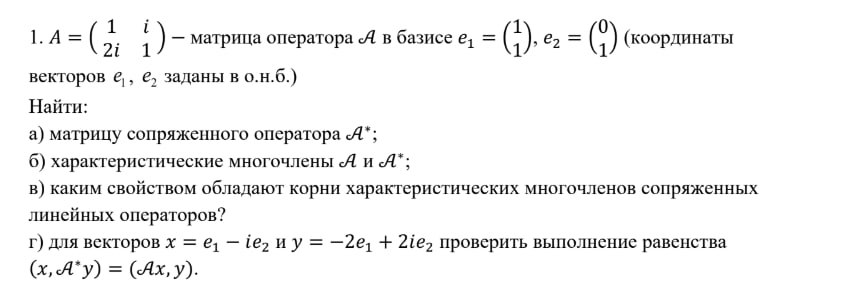
\includegraphics[width = 15 cm]{assets/homework-6-task-1.jpg}
\end{center}
\textbf{Решение:}

\begin{enumerate}
    \item[а)] Сперва найдем матрицу Грама для наших базисных векторов $\Gamma = \begin{pmatrix}
        2 & 1\\
        1 & 1
    \end{pmatrix}$. Чтобы найти матрицу сопряженного оператора воспользуемся формулой: $A^\circledast = \overline{\Gamma^{-1}}\overline{A^T}\overline{\Gamma} = \begin{pmatrix}
        1 & -i\\
        -2i & 1
    \end{pmatrix}$
    \item[б)] Найдем характ многочлен $A$: $\chi_A(t) = (t-1)^2 - (-2) = t^2-2t+3$. Пользуясь свойством 7, так как у нас корни парные(сопряженные), то у $A^*$ такой же характ. 

    \item[в)] корни сопряжены
    \item[г)] Пользуясь формулой скалярного произведения получаю: $-6 -6i = -6-6i$ ура победа!
\end{enumerate}

\subsubsection{Задание 2.}

\begin{center}
   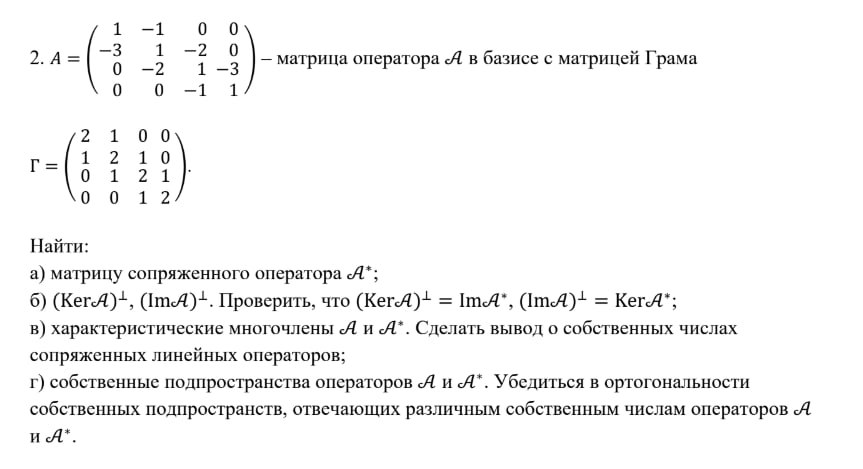
\includegraphics[width = 15 cm]{assets/homework-6-task-2.jpg}
\end{center}
\textbf{Решение:}

\begin{enumerate}
    \item[а)] $A^\circledast = \Gamma^{-1}A^T \Gamma = \begin{pmatrix}
        -1 & -4 & 0 & 1\\
        1 &3 & -3 & -2\\
        -2 & -3 &3 &1\\
        1 & 0  & -4 &-1
    \end{pmatrix}$
    \item[б)] Найдем $\ker A = span\begin{pmatrix}
        -1\\
        -1\\1
        \\1
    \end{pmatrix}$ и $\Im A = \begin{pmatrix}
        1\\
        -3\\0
        \\0
    \end{pmatrix}, \begin{pmatrix}
        -1 \\
        1\\-2\\
        0
    \end{pmatrix}, \begin{pmatrix}
        0\\
        0\\
        -3\\
        1\\
    \end{pmatrix}$. Я устал это делать, в типовике то же самое и я разобрался
\end{enumerate}